\chapter{Exotic pulses}
\label{ch:Exotic}

For a fiber, where $\gamma\neq 0$ and $\betag_2\neq 0$, a pulse launched into it can evolve in a number of surprising ways. Essentially, the nonlinearity will change the local frequency of the pulse based on its power profile, while dispersion will cause different frequencies to advance or delay relative to the carrier frequency, which in turn, alters the power profile. This chapter explores the interplay between these two effects for different values of $\gamma$ and $\betag_2$. 


\section{The Fundamental Soliton}
\label{sec:soliton}
Consider a fiber for which $\gamma>0$. As illustrated in Fig.~\ref{fig:chirp_profiles}, this will cause leading(trailing) pulse edges to develop a red(blue) shift. As explained WHERE?!?!?! $\betag_2<0$ implies that blue light propagates faster than red light, thus causing the leading(trailing) edge of a pulse will become more blue(red). If $\gamma>0$ makes the front(back) of the pulse more red(blue) based on the instantaneous power profile, while $\betag_2<0$ makes the front(back) more blue(red) according to the 2nd time derivative of the field, it's natural to ask if there exists a pulse envelope, where the two effects balance exactly at every instant, so that the shape of the pulse is unaltered as it propagates forward. For such a pulse, the field envelope should be independent of distance, while the phase should be independent of time, such that
\begin{align}
    \A(z,T) &= V(T)e^{i\phi(z)}
\end{align}
solves 
\begin{align}
\label{eq:NLSE_soliton}
    \partial_z\A &=  -i  \frac{\betag_2}{2}\partial_T^2\A+i\gamma|\A|^2\A.
\end{align}
As explained in \href{https://github.com/OleKrarup123/NLSE-vector-solver/blob/main/TutorialVideos/Soliton-Video/Fundamental_soliton_derivation.pdf}{this derivation}, it can be shown that the solution is
\begin{align}
    \A(z,T) &= \sqrt{\frac{|\betag_2|}{\gamma T_0^2}}\cdot\text{sech}\left(\frac{T}{T_0}\right)\exp\left(i\frac{|\betag_2|}{2T_0^2}z\right),
\end{align}
where $T_0$ is the time at which the field of the pulse has decreased to 64.8\% of its peak value. This stable pulse characterized by a hyperbolic secant envelope is referred to as a "fundamental soliton". See Fig.~\ref{fig:gauss_sech} for a comparison of a Gaussian pulse to a hyperbolic-secant pulse. Note that the peak power of the hyperbolic-secant pulse, $\A_{max}$, must be chosen to exactly equal the characteristic amplitude, $\A_{char}=\sqrt{|\betag_2|/\gamma T_0^2}$, for stable propagation to occur!
\begin{figure}
    \centering
    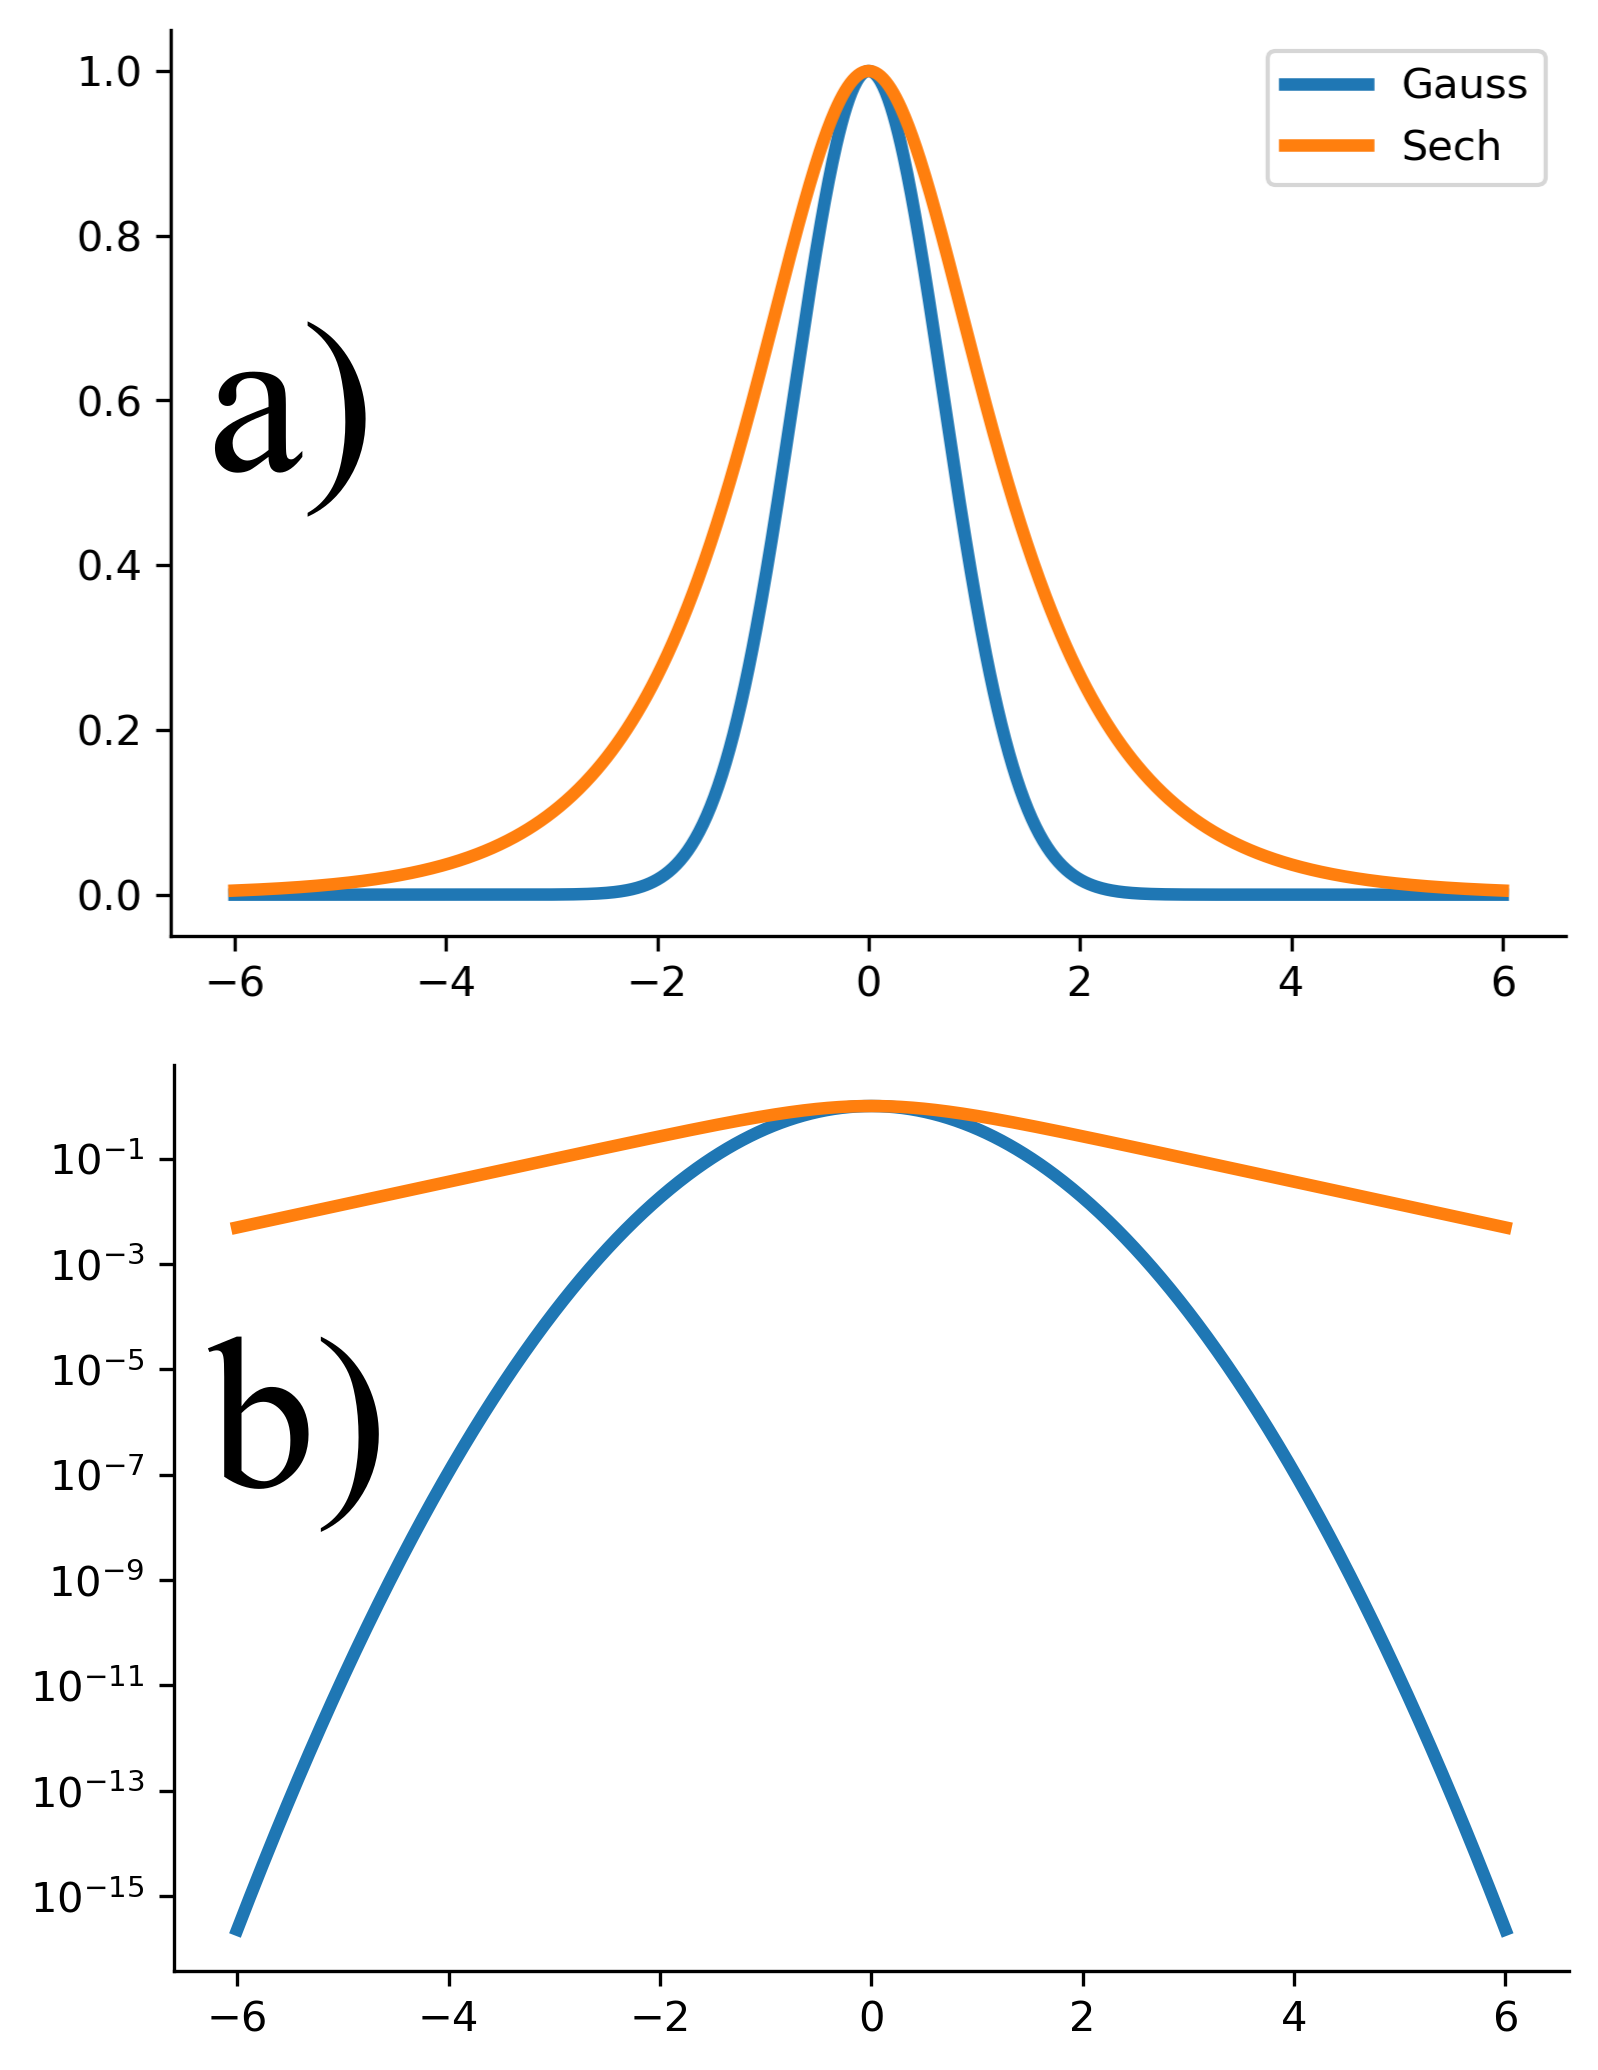
\includegraphics[width=1\linewidth]{figures/gauss_sech_comparison.png}
    \caption{Comparison of a Gaussian pulse to a hyperbolic-secant pulse on a linear scale in a) and a logarithmic scale in b), which emphasizes the comparatively more intense tails of the hyperbolic-secant.  }
    \label{fig:gauss_sech}
\end{figure}
\subsection{Solitons in telecommunications}
As $\gamma>0$ and $\betag_2<0$ in silica fibers for near-infrared frequencies close to 193~THz ($\approx$1550~nm), fundamental solitons were once of great interest in telecommunications because their resistance to dispersion and constant shape reduced inter-symbol interference. However, the same improvements in electronic dispersion compensation mentioned in Subsection~\ref{subsec:ZDF} have rendered the use of solitons for optical fiber communication obsolete. Instead, pulses with a so-called "\href{https://www.youtube.com/watch?v=Qe8NQx4ibE8}{root-raised-cosine}" field envelope are used.   


\section{Higher order Solitons}
If the peak power of the hyperbolic secant pulse smaller than $P_{char}=|\A_{char}|^2=|\betag_2|/\gamma T_0^2$, the nonlinear effect will be too weak compared to dispersion for a fundamental soliton to form. The pulse wivll thus simply broaden in the time domain as it propagates forward. If the peak power is increased beyond $P_{char}$, the pulse will exhibit "oscillations" as it evolves. For the special cases of $\A_{max}$ being an integer multiple of $\A_{char}$, the oscillating soliton evolution will be particularly well-behaved. See Fig.~\ref{fig:Soliton_comparison}~a-b) for an example of the temporal and spectral evolutions of a soliton for which $\A_{max}=3\A_{char}$. See \href{https://youtu.be/KAZ7pCQ-x8Y}{this video tutorial} for more information on solitons in fibers. 

\subsection{Soliton fission}
\label{subsec:fission}
Fundamental- and higher order solitons can be seen as "fixed points" of Eq.~\ref{eq:NLSE_soliton}. However, Eq.~\ref{eq:NLSE_soliton} itself is only an approximation to Eq.~\ref{eq:GNLSE}, which provides a more general description of the physics affecting the propagation of an optical pulse in a dispersive and nonlinear medium. It turns out that the presence of effects other than $\gamma>0$ and $\betag_2<0$ will eventually disturb the evolution of an initially solitonic pulse. In Fig.\ref{fig:Soliton_comparison}~c-d), the presence of $\betag_3>0$ causes a higher order soliton to "fission" into two less powerful ones at new frequencies due to FWM after propagating a distance of 0.5 meters. Other effects, such as Self-Steepening, the Raman effect or even Modulation Instability caused by optical noise propagating along with an otherwise ideal soliton pulse can similarly give rise to soliton fission. Thus, much like a pencil balanced on its tip, solitonic propagation should be viewed as an unstable equilibrium. See \href{https://youtu.be/tHpIR2Kuxp0}{this video tutorial} for more details on soliton fission.
\begin{figure}
    \centering
    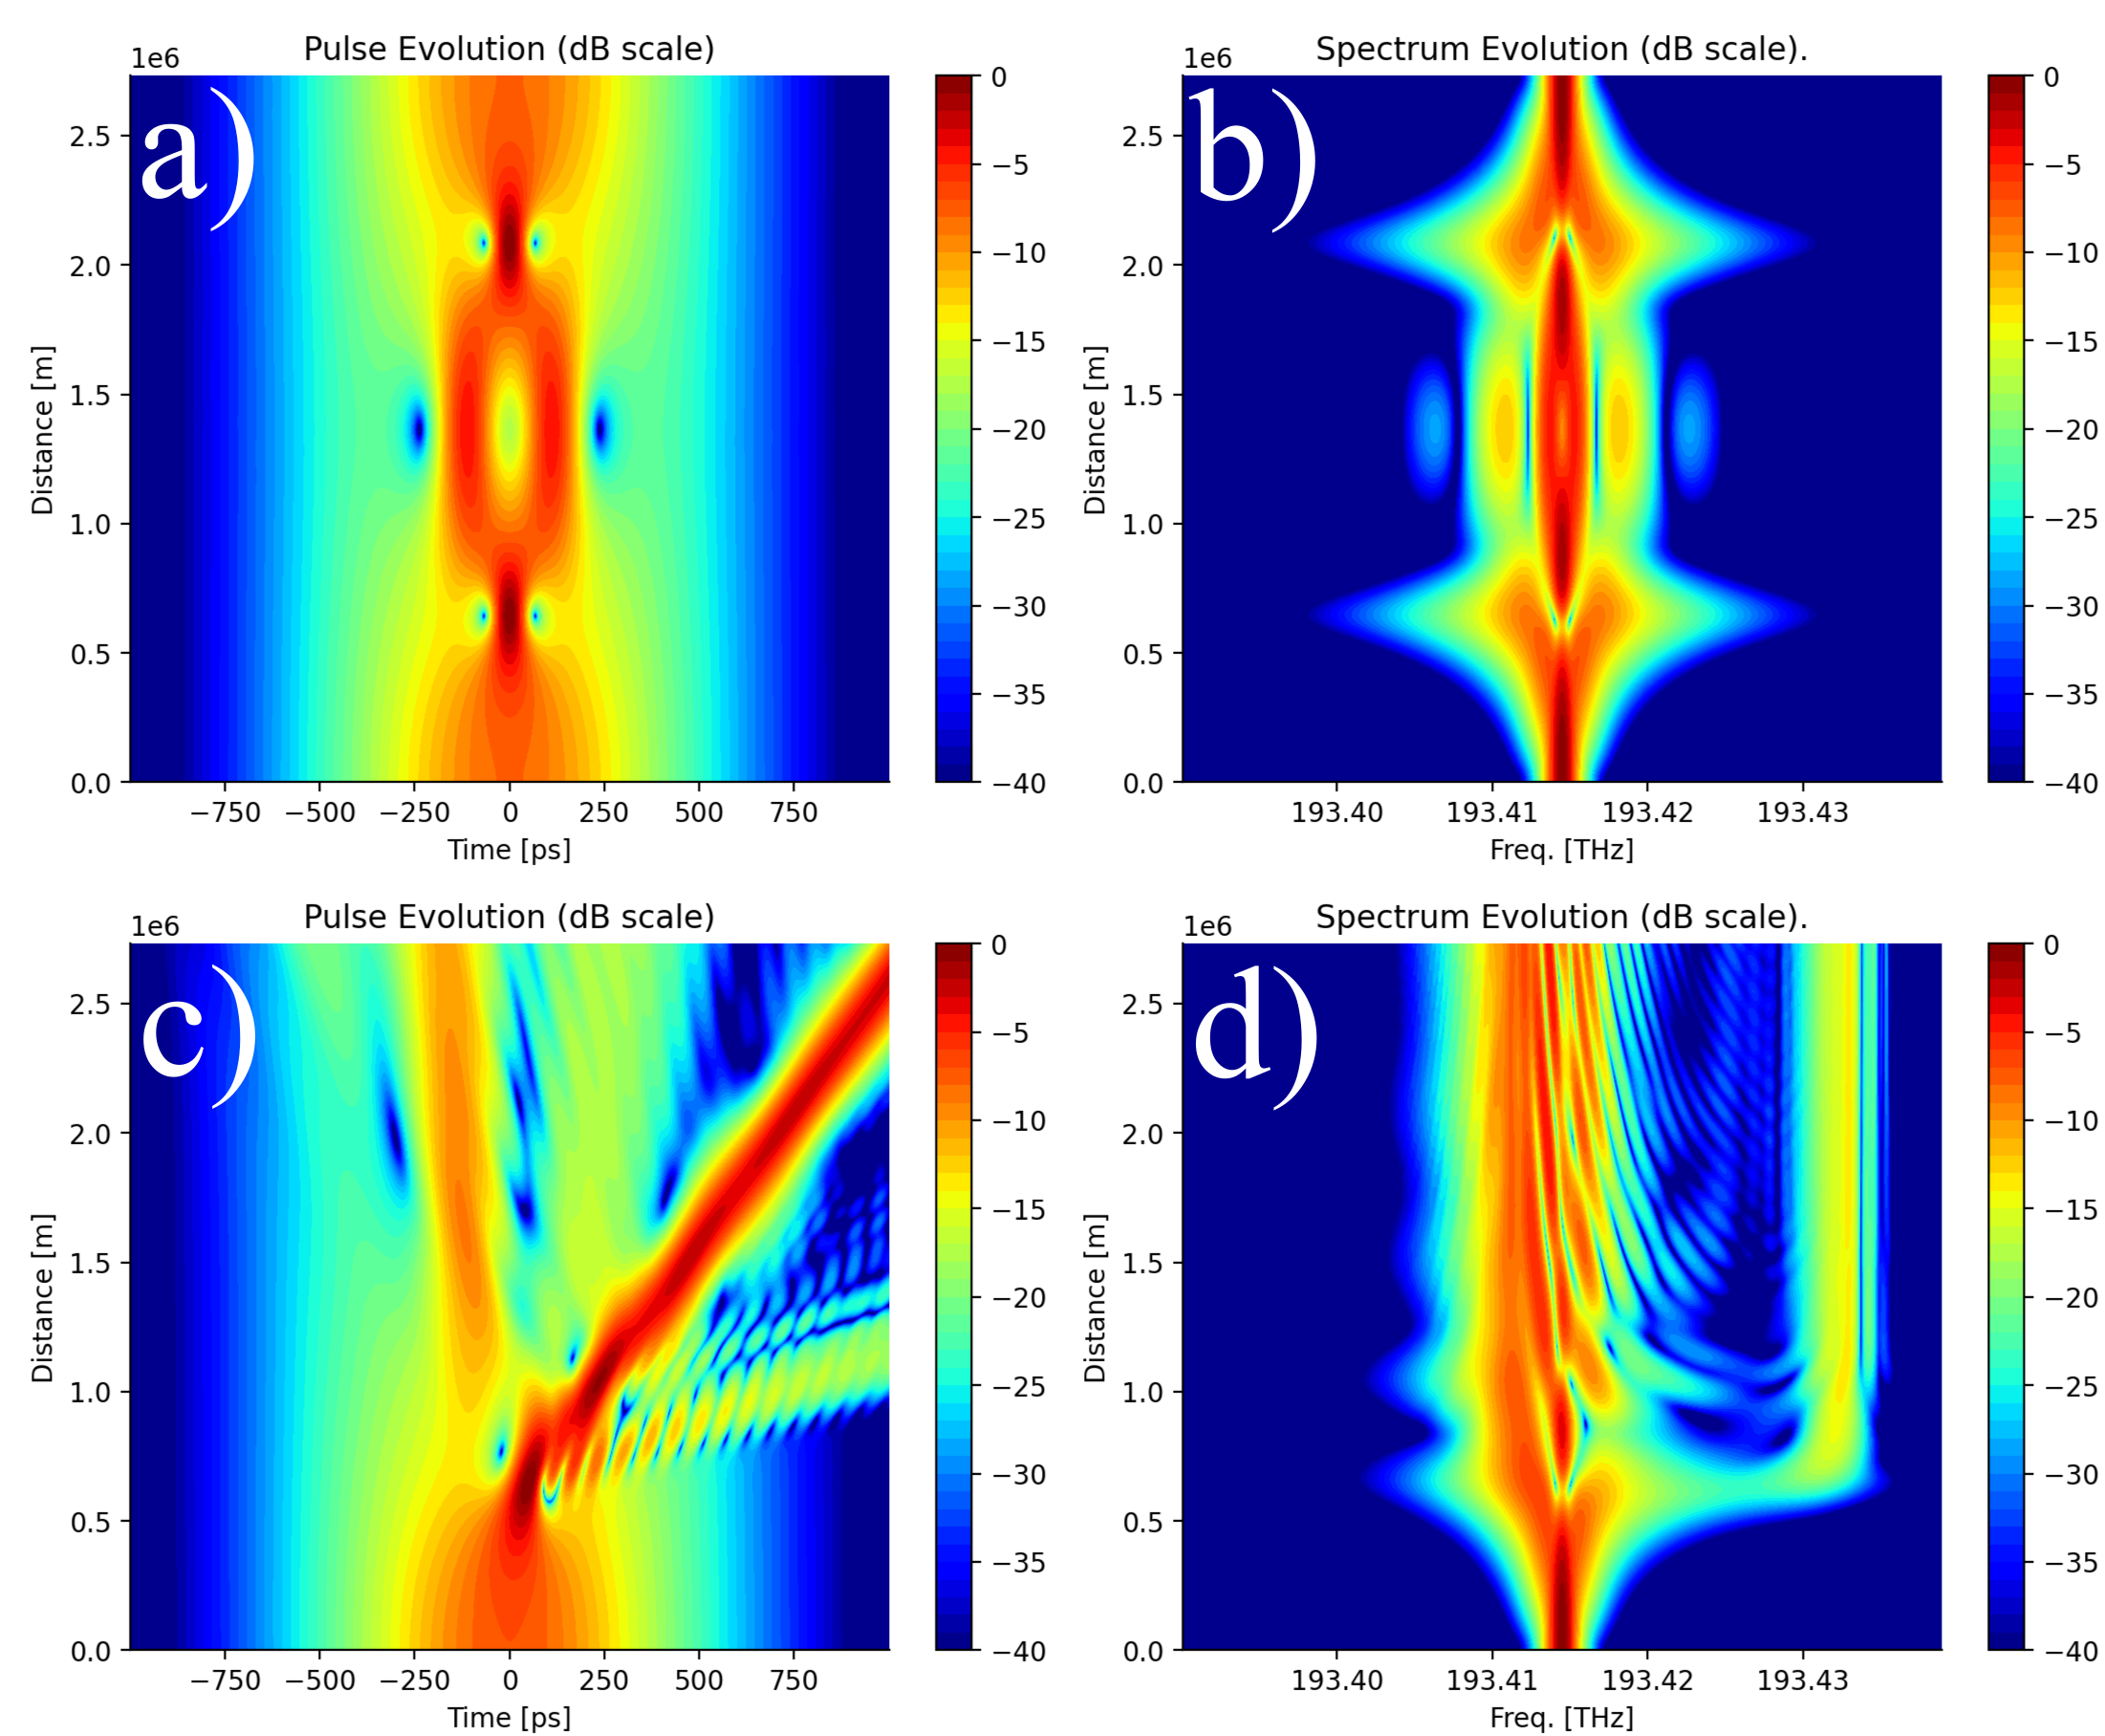
\includegraphics[width=1\linewidth]{figures/Soliton_comparison.png}
    \caption{a) Temporal evolution of an $N=3$ soliton for which $\A_{max}=3\A_{char}=3\sqrt{|\betag_2|/\gamma T_0^2}$. The length of the fiber has been chosen to equal the oscillation period of the soliton. b) Spectrum evolution of the $N=3$ soliton. c-d) Respectively, the temporal and spectral evolutions of the same $N=3$ soliton as in a-b), but where the fiber has $\betag_3>0$, causing the pulse to "fission", thereby illustrating the unstable nature of solitonic propagation. Figures generated using the numerical simulation in \href{https://colab.research.google.com/drive/123pT-IsLWIEZY9XW3-1WzkTXfg1IEkkD?usp=sharing}{this interactive notebook}, which the reader is encouraged to experiment with.}
    \label{fig:Soliton_comparison}
\end{figure}





\section{Optical Wave Breaking}
When an ocean wave approaches a beach, water begins to "pile up" on its leading edge, eventually causing the wave to "break" before crashing onto the shore. A similar phenomenon can be observed with optical waves in nonlinear fibers where $\gamma>0$ and $\betag_2>0$. Instead of the local color-changes from nonlinearity and dispersion balancing as in Sec.~\ref{sec:soliton} when $\betag_2$ was negative, they now "cooperate". The nonlinearity makes the front(back) of the pulse more red(blue) and dispersion causes red(blue) light to move faster(slower) than the carrier. The result is that any pulse will quickly broaden in the time domain. Often, this happens in such a way that power gradually "piles up" in both the front and back of the pulse, leading to steeper power slopes, which generate even larger chirps causing more rapid temporal broadening due to dispersion. When the slope steepness gets sufficiently large, dispersion will "launch" the newly generated frequencies away from the main pulse in a manner analogous to a crashing water wave. Figure~\ref{fig:OWB_and_similariton}~a-b) illustrates this effect called "Optical Wave Breaking" (OWB). While the changes to incident pulses induced by OWB can be detrimental, they can also be beneficial if one desires an optical pulse with steep slopes and approximately constant peak power. See \href{https://youtu.be/XEx6lOf6f40}{this video tutorial} for further details on OWB. 

\subsection{Similaritons}
When $\gamma>0$ and $\betag_2>0$, OWB broadens the pulse in the time domain, thereby reducing its peak power. If, additionally, $\alpha>0$, implying that the pulse is amplified as it moves forward, this loss of peak power is continuously replaced. It turns out that under these circumstances, any input pulse \emph{regardless of its initial shape} will evolve towards a parabolic power envelope as illustrated in Fig.~\ref{fig:OWB_and_similariton}~c) and a linearly changing chirp that goes from red in the front to blue in the back\cite{Similariton_evolution}. Both the peak power and duration of such a "similarition" will continuously increase with distance as explained in \href{https://youtu.be/ZtWIRaj5VV4}{this video tutorial}. Similaritons can arise in certain optical amplifiers and their linearly changing chirps make them ideal candidates for generating pulses with extremely high peak powers through the Nobel-Prize winning method of chirped pulse compression explained in \href{https://youtu.be/Eh5CHRWFT-M}{this video tutorial}.   

\begin{figure}
    \centering
    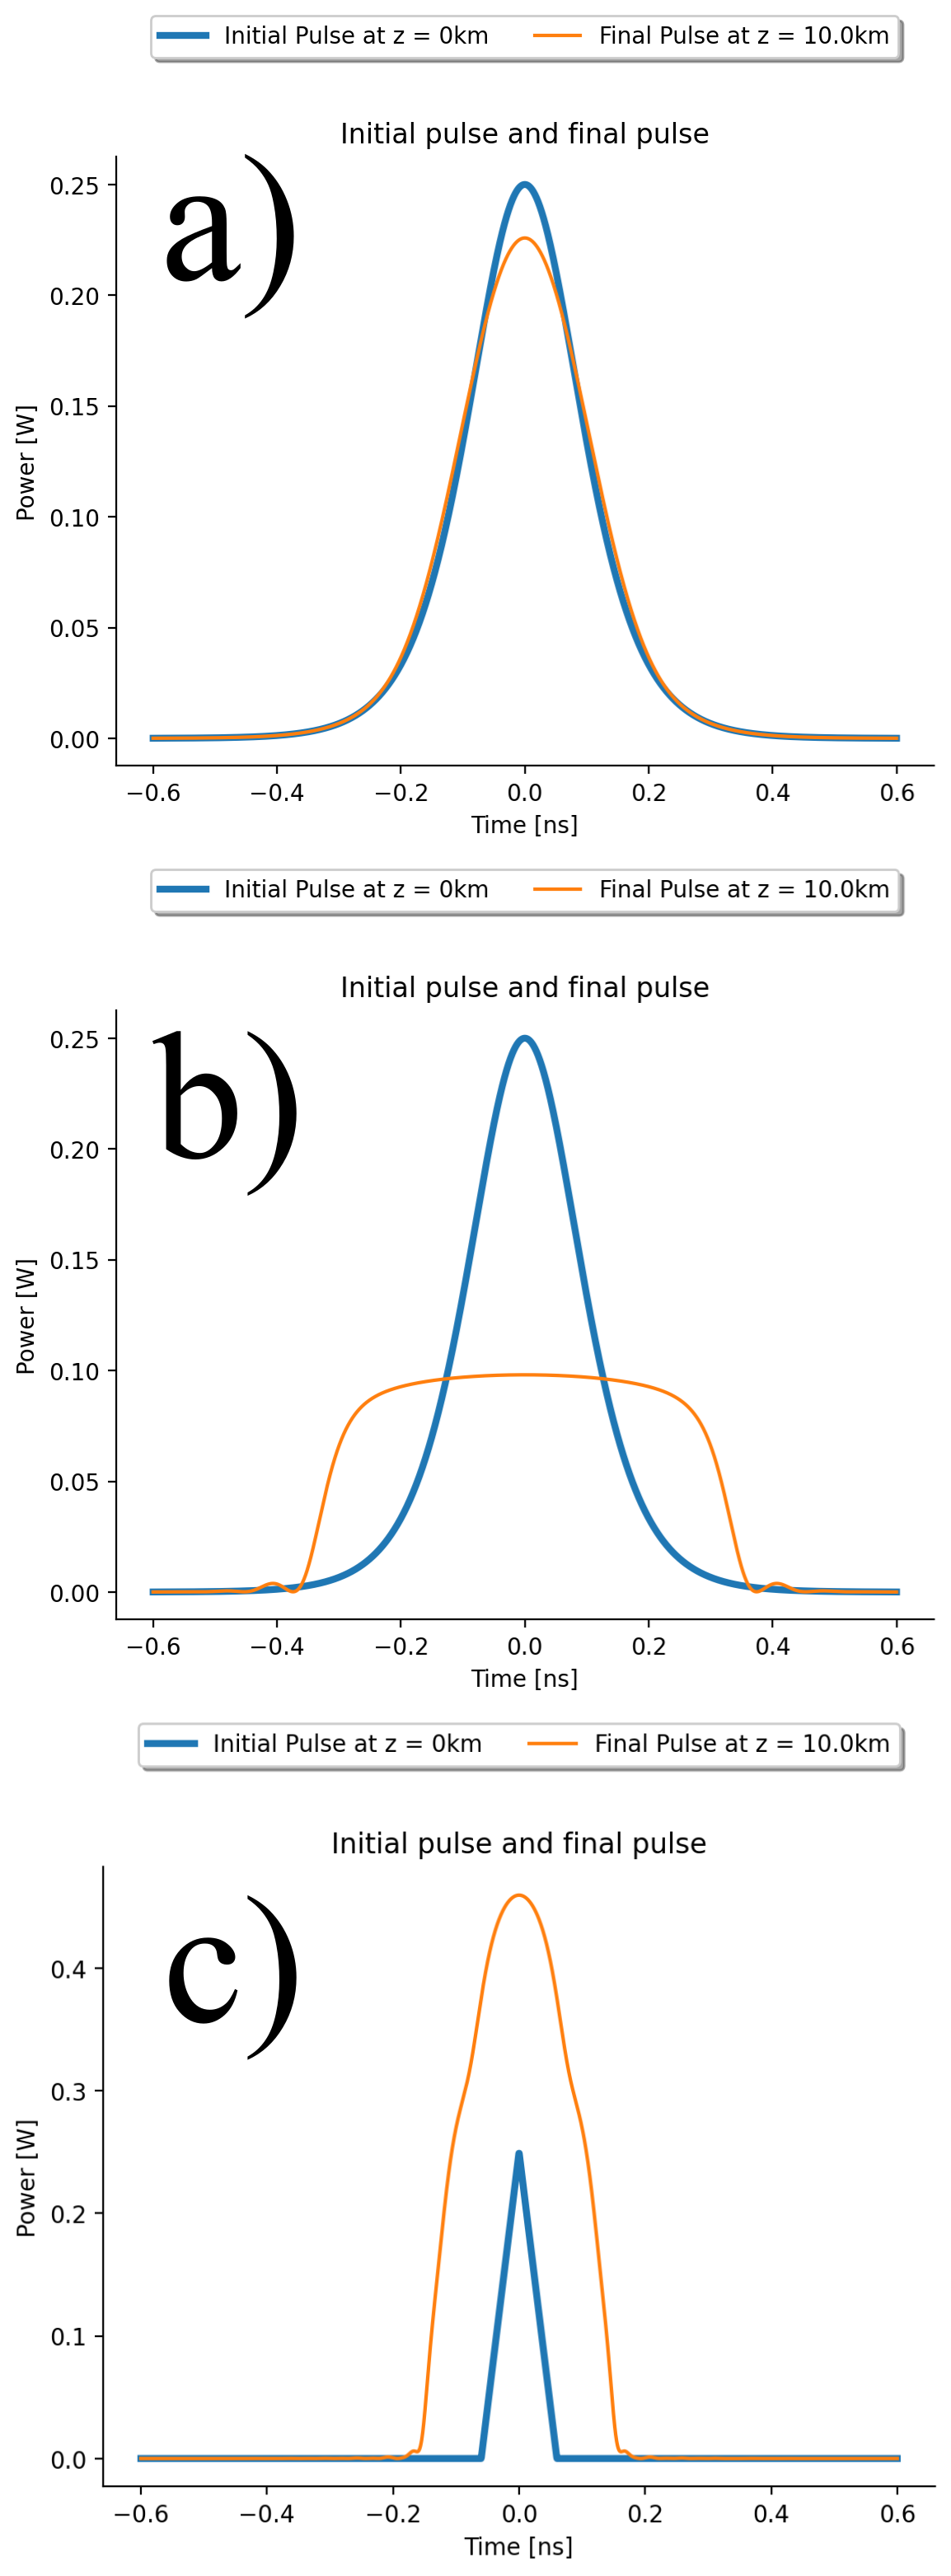
\includegraphics[width=0.57\linewidth]{OWB_and_similariton.png}
    \caption{a) Evolution of a triangular pulse through a medium where $\betag_2>0$. b) Evolution of the same pulse as in a) through a medium where $\betag_2>0$ and $\gamma>0$ causes power to "pile up" in the front and back of the pulse. c) Same conditions as in b), but where $\alpha>0$ causes the triangular pulse to evolve towards a parabola. Figures generated using the numerical simulation in \href{https://colab.research.google.com/drive/1qtMcXElXn4VBntfCgXIGGkyDfiGicElx?usp=sharing}{this interactive notebook}, which the reader is encouraged to experiment with.  }
    \label{fig:OWB_and_similariton}
\end{figure}


\section{Novel Solitons}
\subsection{Dark Solitons} 
Typically, optical pulses consist of a sudden increase in laser power preceded and followed by long durations of zero power. To the naked eye, such a pulse would be a bright flash, like a lamp being briefly switched on in a dark room. Such pulses can propagate stably through a nonlinear medium if the conditions described in Sec.~\ref{sec:soliton} are satisfied. Consider instead what might be called an "anti-pulse" in a nonlinear medium; a high power CW signal, which experiences a brief dip in its power, analogous to a bright lamp that is briefly switched off before being reactivated. It will consist of a decreasing leading edge and an increasing trailing edge. If $\gamma>0$ and $\betag_2>0$, the leading(trailing) edge becomes more blue(red), causing the light there to slow down(speed up). Similarly to Sec.~\ref{sec:soliton}, one can calculate that the field envelope for which nonlinearity and dispersion cancel exactly is a hyperbolic tangent, thereby leading to a stably propagating "Dark Soliton" described by 
\begin{align}
    \A(z,T) = \A_{char}\tanh\left(\frac{T}{T_0}\right)\exp\left(i\frac{|\betag_2|}{T_0^2}z \right).
\end{align}
See \href{https://youtu.be/MrNfI1_eTZ0}{this video tutorial} for more information on Dark Solitons.


\subsection{Raman Solitons}
If the Raman effect, which shifts the spectrum of a pulse towards lower frequencies, is present in a nonlinear medium where $\betag_2<0$, a "Raman Soliton" can form. This soliton retains the shape of its envelope, but undergoes a constant red-shift and obtains an increasingly large time delay since $\betag_2<0$ implies that red light moves more slowly than blue light as illustrated in Fig.~\ref{fig:dark_and_raman}c-d). Raman solitons often arise after soliton fission of pulses with durations on the scale of tens of femtoseconds. See \href{https://www.youtube.com/watch?v=K33YUfegL1w}{this video tutorial} for an explanation of Raman solitons.

\begin{figure}
    \centering
    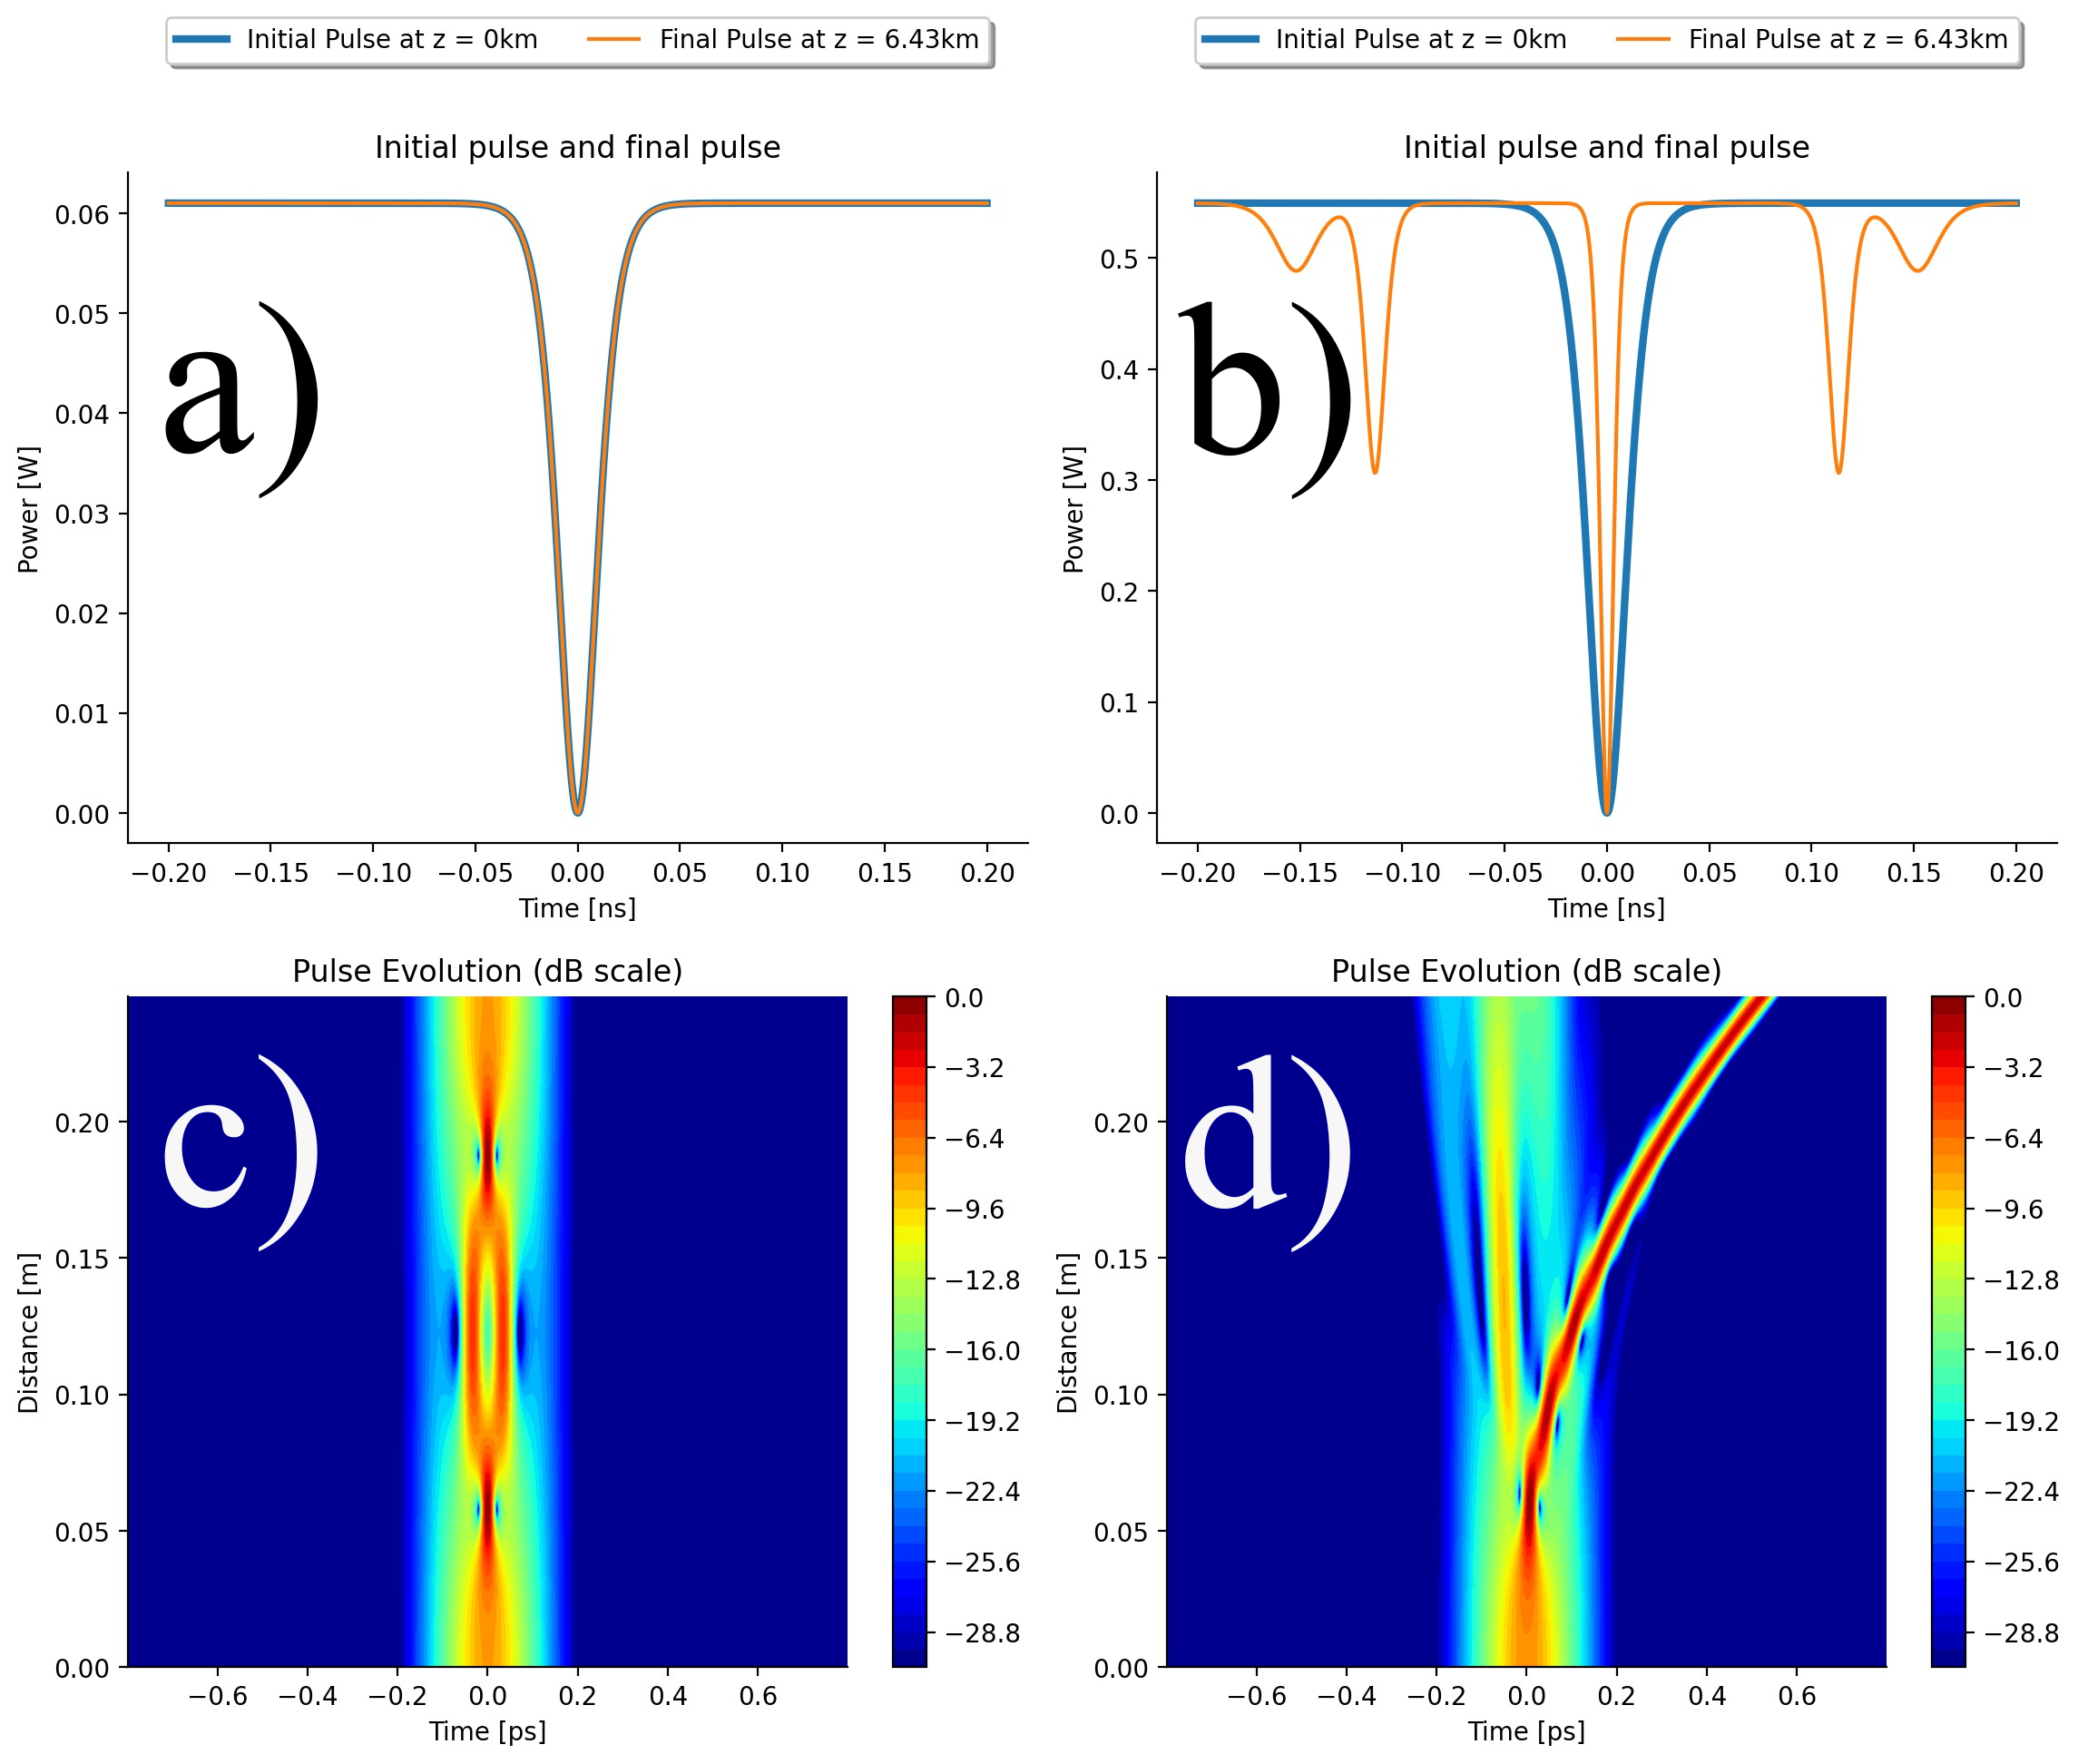
\includegraphics[width=1\linewidth]{figures/dark_and_raman_soliton_combined.png}
    \caption{a) Fundamental dark soliton propagating stably through a medium where $\betag_2>0$ and $\gamma>0$. b) An N=3 dark soliton propagating through the same medium as in a) Instead of stable propagation, the central dip gives rise to additional ones. c) An N=3 soliton propagating through a medium where $\betag_2<0$ and $\gamma>0$. d) The same pulse as in c) propagating through the same medium except the Raman effect described by Eq.~\ref{eq:raman_basic} is taken into account, causing soliton fission and a self-redshifting Raman soliton to arise.  }
    \label{fig:dark_and_raman}
\end{figure}

\subsection{Vector Solitons}
In Sec.~\ref{Sec:XPM}, it was shown that two distinct frequencies of light can affect each others phases through the nonlinearity. Similarly, two different polarizations of light propagating in a nonlinear medium can affect each other's phases. Using a vectorial version of Eq.\ref{eq:GNLSE} where $\gamma>0$, $\betag_2<0$, and where the refractive index is different for light polarized along the x- and y-axes of the medium, one can obtain analytical expressions for so-called "Vector Solitons". The special cases for which this is possible turn out to be circularly polarized light and light polarized linearly at $45^{o}$ to the x-axis. See AGRAWAL!?!?!?! for more details. 






